\documentclass[aspectratio=43,11pt]{beamer}
\usetheme{default}
\setbeamertemplate{navigation symbols}{}
\setbeamertemplate{footline}[frame number]
\usepackage{amsmath,amssymb}
\usepackage{booktabs}
\usepackage{tikz}
\usepackage{pgfplots}
\pgfplotsset{compat=1.16}
\usepackage{xcolor}
\definecolor{maroon}{HTML}{500000}
\setbeamercolor{structure}{fg=maroon}
\usepackage{listings}
\lstset{basicstyle=\ttfamily\scriptsize,columns=fullflexible,keepspaces=true}
\newcommand{\nb}[1]{\tikz[remember picture,overlay]\node[anchor=north east,font=\scriptsize,text=gray] at ([xshift=-0.3cm,yshift=-0.25cm]current page.north east) {Notebook: Part #1};}
\newcommand{\question}[1]{\begin{alertblock}{The question}#1\end{alertblock}}
\newcommand{\answer}[1]{\begin{exampleblock}{The answer}#1\end{exampleblock}}

\title{Principal Component Analysis (PCA)}
\author{DAEN 300 - Fall 2026}
\date{}
\titlegraphic{\IfFileExists{TAMU_logo.png}{
\includegraphics[height=1.2cm]{TAMU_logo.png}}{}}

\begin{document}

% ------------------------------------------------------------
\begin{frame}
  \titlepage
\end{frame}

% ------------------------------------------------------------
\begin{frame}{Assignment}
  \begin{itemize}
    \item The assignment is due next Friday before class.
    \item It's not graded, just marked completed as satisfactory/unsatisfactory, so don't stress.
    \item That said, use it to study, because we'll start class with a short, multiple-choice quiz on the same material.
    \item Be sure to arrive on time so you don't miss any of the quiz!
  \end{itemize}
  \vspace{1em}
  {\bf IMPORTANT}\\Heads up \rightarrow~Fri Nov 20 and Tue Dec 1 (redefined day), we’ll build a mini project in class.
  Please make sure you don’t miss these sessions!
  If you miss either session, you'll make it up on final exam day. If you attend both, you're done: Dec 1 will be our last class!
\end{frame}

% ------------------------------------------------------------
\begin{frame}{Why PCA?}
  \begin{itemize}
    \item Real data often has \textbf{many columns}: sensors, pixels, metrics.
    \item Many columns tell the same story. They go up and down together.
    \item PCA replaces them with a \textbf{few new columns} that keep most of the information.
  \end{itemize}
  \vspace{0.8em}
  \textbf{What it is used for:}
  \begin{itemize}
    \item Shrinking data (64 columns $\to$ 2)
    \item Plotting data that has too many columns to draw
    \item Removing noise
    \item Preparing inputs for a model
  \end{itemize}
  \vspace{0.5em}
  PCA does not use labels. It only looks at the numbers.
\end{frame}

% ------------------------------------------------------------
\begin{frame}{}
Students usually struggle with PCA in three areas:
\begin{itemize}
  \item \textbf{Interpreting} the results
  \item The \textbf{mathematical intuition} behind the method
  \item Knowing \textbf{when to apply} the technique
\end{itemize}
\end{frame}

% ------------------------------------------------------------
% \section{1.\ What do the Principal Components actually mean?}

\begin{frame}{1. What do the Principal Components (PCs) actually mean?}
This is the biggest difficulty. Because PCA creates new variables as
\textbf{linear combinations} of the original ones, the original physical
meaning is lost.

\question{If PC1 is a mix of \emph{age}, \emph{salary}, and \emph{credit score},
how do I explain to the client or the business what PC1 represents?}

\answer{Look at the \textbf{loadings} of each original variable on the component.
If \emph{salary} and \emph{credit} have very high weights on PC1, students learn
to interpret PC1 informally as \textbf{``Purchasing Power.''}}
\end{frame}

% ------------------------------------------------------------
% \section{2.\ How many components should I keep?}

\begin{frame}{2. How many Principal Components should I choose?}
\question{If I had 20 variables and PCA produced 20 components,
how many should I keep in my model?}

\answer{Students often confuse the different criteria. The usual approaches are:
\begin{itemize}
  \item The \textbf{elbow plot} (\emph{scree plot})
  \item Keeping the components that together account for
        \textbf{70\%--90\% of the total explained variance}
\end{itemize}}
\end{frame}

% ------------------------------------------------------------
% \section{3.\ Why standardize the data?}

\begin{frame}[fragile]{3. Why is it mandatory to standardize (scale) the data?}
\question{What happens if I forget to use \texttt{StandardScaler} (in Python)?}

\answer{PCA is extremely \textbf{sensitive to scale}.
\begin{itemize}
  \item Height in meters: roughly 1 to 3
  \item Salary: roughly \$2{,}000 to \$10{,}000
\end{itemize}
PCA will put almost 100\% of its attention on the variable with larger numbers
(salary), treating it as having more variation and ignoring the importance of
the other. Standardizing gives every variable \textbf{mean 0 and variance 1}.}
\end{frame}

% ------------------------------------------------------------
% \section{4.\ Categorical variables}

\begin{frame}{4. Does PCA work for categorical variables (text/classes)?}
\question{Can I apply PCA to columns such as \emph{Gender},
\emph{Marital Status}, or \emph{Car Type}?}

\answer{\textbf{Not directly.} Traditional PCA was designed strictly for
\textbf{continuous numerical data}, since it relies on covariance and
Euclidean distance.

For categorical data, students find they need variant techniques such as:
\begin{itemize}
  \item \textbf{Multiple Correspondence Analysis (MCA)}
  \item \textbf{Factor Analysis of Mixed Data (FAMD)}
\end{itemize}}
\end{frame}

% ------------------------------------------------------------
% \section{5.\ Is PCA a predictive model?}

\begin{frame}{5. Does PCA help predict better? Is it a predictive model?}
\question{Can I use PCA to predict the price of a house?}

\answer{\textbf{No.} PCA does not predict anything on its own; it is an
\textbf{unsupervised learning} algorithm.

It only \emph{tidies up the house}: it cleans and compresses the data so that
another algorithm (such as a \textbf{Regression} or a \textbf{Decision Tree})
can make the prediction faster and more efficiently.}
\end{frame}




% ------------------------------------------------------------
\begin{frame}{The idea in one picture}
  \centering
  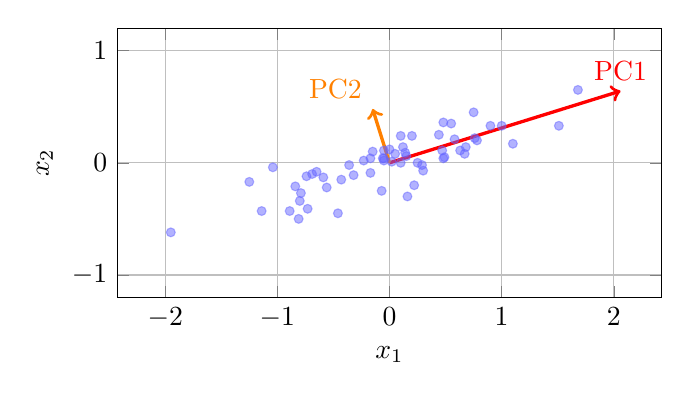
\begin{tikzpicture}
    \begin{axis}[width=8.5cm,height=5cm,axis equal,
        xmin=-2.3,xmax=2.3,ymin=-1.2,ymax=1.2,
        xlabel={$x_1$},ylabel={$x_2$},grid=major]
      \addplot[only marks,mark=*,blue!60,opacity=0.5,mark size=1.6pt] coordinates {
(0.12,0.14)(-0.69,-0.10)(0.68,0.14)(-1.04,-0.04)(1.51,0.33)(0.75,0.45)(1.68,0.65)(-1.14,-0.43)(-0.46,-0.45)(-1.25,-0.17)(-0.05,0.04)(0.44,0.25)(0.67,0.08)(-1.95,-0.62)(-0.32,-0.11)(0.20,0.24)(0.15,0.06)(0.76,0.22)(-0.65,-0.08)(0.30,-0.07)(0.48,0.04)(0.47,0.11)(0.49,0.05)(-0.23,0.02)(-0.56,-0.22)(-0.15,0.10)(-0.05,0.02)(1.00,0.33)(0.55,0.35)(-0.06,0.04)(-0.59,-0.13)(-0.84,-0.21)(-0.00,0.12)(0.02,0.01)(-0.74,-0.12)(0.10,0.00)(0.22,-0.20)(0.78,0.20)(-0.43,-0.15)(0.48,0.36)(-0.05,0.11)(1.10,0.17)(-0.80,-0.34)(-0.17,0.04)(0.58,0.21)(0.16,-0.30)(-0.17,-0.09)(0.25,-0.00)(-0.89,-0.43)(0.05,0.08)(0.10,0.24)(-0.79,-0.27)(0.14,0.09)(-0.73,-0.41)(0.29,-0.02)(-0.81,-0.50)(0.90,0.33)(0.63,0.11)(-0.36,-0.02)(-0.07,-0.25)};
      \draw[->,very thick,red] (axis cs:0,0) -- (axis cs:2.06,0.64) node[above]{PC1};
      \draw[->,very thick,orange] (axis cs:0,0) -- (axis cs:-0.15,0.48) node[above left]{PC2};
    \end{axis}
  \end{tikzpicture}

  \raggedright
  \begin{itemize}
    \item The points lie close to a line.
    \item \textbf{PC1} points along that line, where the data spreads the most.
    \item \textbf{PC2} is at a right angle to PC1 and holds the small leftover spread.
    \item We can describe each point mostly by \emph{where it falls along PC1}.
  \end{itemize}
\end{frame}

% ------------------------------------------------------------
\begin{frame}{The recipe}
  \begin{enumerate}
    \item \textbf{Center}: subtract each column's average.
    \item \textbf{Covariance}: measure how the columns spread and move together.
    \item \textbf{Eigenvectors and eigenvalues} of the covariance matrix:
      \begin{itemize}
        \item eigenvector = a new direction (an axis)
        \item eigenvalue = how much the data spreads along it
      \end{itemize}
    \item \textbf{Sort} the directions, biggest spread first.
    \item \textbf{Project}: find each point's position along the new axes.
          Keep only the first few.
  \end{enumerate}
  \vspace{0.8em}
  \[
    C = \frac{1}{n-1} X_c^\top X_c \qquad\qquad C\,v = \lambda\,v
  \]
\end{frame}

% ------------------------------------------------------------
\begin{frame}{Example: two temperature sensors \nb{1}}
  Two sensors on the same machine, five readings.
  \vspace{0.3em}
  \begin{columns}[c]
    \column{0.38\textwidth}
    \centering
    \begin{tabular}{ccc}
      \toprule
      Reading & $x_1$ & $x_2$ \\
      \midrule
      1 & 1 & 2 \\
      2 & 2 & 1 \\
      3 & 3 & 3 \\
      4 & 4 & 5 \\
      5 & 5 & 4 \\
      \midrule
      Average & 3 & 3 \\
      \bottomrule
    \end{tabular}
    \column{0.62\textwidth}
    \centering
    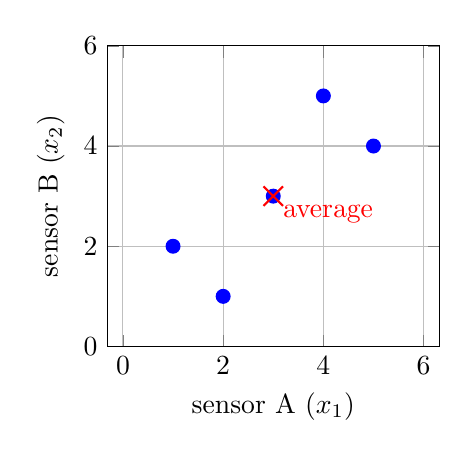
\begin{tikzpicture}
      \begin{axis}[width=5.8cm,height=5.4cm,axis equal,
          xmin=0,xmax=6,ymin=0,ymax=6,
          xlabel={sensor A ($x_1$)},ylabel={sensor B ($x_2$)},grid=major]
        \addplot[only marks,mark=*,blue,mark size=2.5pt]
          coordinates {(1,2)(2,1)(3,3)(4,5)(5,4)};
        \addplot[only marks,mark=x,red,mark size=5pt,thick]
          coordinates {(3,3)};
        \node[red,below right] at (axis cs:3,3) {average};
      \end{axis}
    \end{tikzpicture}
  \end{columns}
  \vspace{0.5em}
  The sensors mostly agree: when A reads high, B reads high too.
\end{frame}

% ------------------------------------------------------------
\begin{frame}{Steps 1--2: center and covariance \nb{1}}
  \textbf{Center:} subtract the average $(3,3)$ from every reading.
  \[
    X_c = \begin{pmatrix}
      -2 & -1 & 0 & 1 & 2\\ -1 & -2 & 0 & 2 & 1
    \end{pmatrix}^{\!\top}
  \]
  \textbf{Covariance:} multiply, add up, divide by $n-1 = 4$.
  \begin{align*}
    \text{spread of } x_1 &= \tfrac{4+1+0+1+4}{4} = 2.5\\[2pt]
    \text{spread of } x_2 &= \tfrac{1+4+0+4+1}{4} = 2.5\\[2pt]
    \text{moving together} &= \tfrac{2+2+0+2+2}{4} = 2.0
  \end{align*}
  \[
    C = \begin{pmatrix} 2.5 & 2.0 \\ 2.0 & 2.5 \end{pmatrix}
    \qquad \text{total spread} = 2.5 + 2.5 = 5.0
  \]
\end{frame}

% ------------------------------------------------------------
\begin{frame}{Step 3: eigenvalues and eigenvectors \nb{1}}
  Solve $\det(C - \lambda I) = 0$:
  \[
    (2.5-\lambda)^2 - 2^2 = 0
    \;\Rightarrow\; 2.5 - \lambda = \pm 2
    \;\Rightarrow\; \boxed{\lambda_1 = 4.5,\;\; \lambda_2 = 0.5}
  \]
  The matching directions (length 1):
  \[
    v_1 = \tfrac{1}{\sqrt2}\begin{pmatrix}1\\1\end{pmatrix}
    \qquad
    v_2 = \tfrac{1}{\sqrt2}\begin{pmatrix}1\\-1\end{pmatrix}
  \]
  \textbf{Check:} $C v_1 = \tfrac{1}{\sqrt2}(4.5,\;4.5)^\top = 4.5\,v_1$ \checkmark
  \vspace{0.6em}
  \begin{itemize}
    \item $4.5 + 0.5 = 5.0$: the same total spread, just on new axes.
    \item PC1 $(1,1)$: both sensors together, i.e.\ the \emph{shared} temperature.
    \item PC2 $(1,-1)$: how much the sensors \emph{disagree}.
  \end{itemize}
\end{frame}

% ------------------------------------------------------------
\begin{frame}{How much does each direction hold? \nb{1}}
  \begin{columns}[c]
    \column{0.5\textwidth}
    Share of the total spread:
    \[
      \frac{\lambda_k}{\lambda_1 + \lambda_2}
    \]
    \begin{tabular}{lcc}
      \toprule
      & $\lambda$ & share \\
      \midrule
      PC1 & 4.5 & \textbf{90\%} \\
      PC2 & 0.5 & 10\% \\
      \bottomrule
    \end{tabular}
    \column{0.5\textwidth}
    \centering
    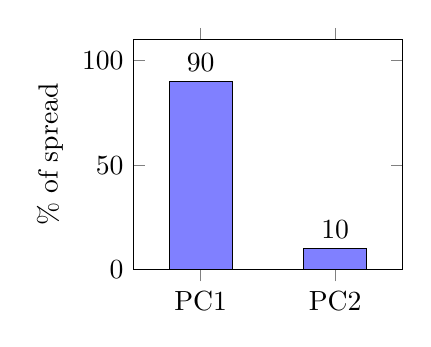
\begin{tikzpicture}
      \begin{axis}[ybar,width=5cm,height=4.5cm,ymin=0,ymax=110,ytick={0,50,100},
          symbolic x coords={PC1,PC2},xtick=data,
          ylabel={\% of spread},nodes near coords,bar width=0.8cm,
          enlarge x limits=0.5]
        \addplot[fill=blue!50] coordinates {(PC1,90)(PC2,10)};
      \end{axis}
    \end{tikzpicture}
  \end{columns}
  \vspace{1em}
  One number per reading (instead of two) keeps 90\% of the information.
  This is called the \textbf{explained variance ratio}.
\end{frame}

% ------------------------------------------------------------
\begin{frame}{Steps 4--5: new coordinates \nb{1}}
  Each reading's position along the new axes (its \textbf{score}):
  \[
    z_1 = \frac{x_{c1} + x_{c2}}{\sqrt2} \qquad z_2 = \frac{x_{c1} - x_{c2}}{\sqrt2}
  \]
  \begin{center}
  \begin{tabular}{cccc}
    \toprule
    Reading & centered & $z_1$ & $z_2$ \\
    \midrule
    1 & $(-2,-1)$ & $-2.12$ & $-0.71$ \\
    2 & $(-1,-2)$ & $-2.12$ & $\phantom{-}0.71$ \\
    3 & $(\phantom{-}0,\phantom{-}0)$ & $\phantom{-}0.00$ & $\phantom{-}0.00$ \\
    4 & $(\phantom{-}1,\phantom{-}2)$ & $\phantom{-}2.12$ & $-0.71$ \\
    5 & $(\phantom{-}2,\phantom{-}1)$ & $\phantom{-}2.12$ & $\phantom{-}0.71$ \\
    \bottomrule
  \end{tabular}
  \end{center}
  \textbf{Check:}spread of $z_1$ is $4.5$ and spread of $z_2$ is $0.5$ (eigenvalues \checkmark)

  \vspace{0.3em}
  {\footnotesize Software may flip the sign of a direction. The scores flip too; nothing else.}
\end{frame}

% ------------------------------------------------------------
\begin{frame}{Keep only PC1 \nb{1}}
  \begin{columns}[c]
    \column{0.48\textwidth}
    Drop $z_2$ and rebuild each reading from $z_1$ alone:
    \[
      \hat{x} = \text{average} + z_1\, v_1
    \]
    Reading 1:\\
    $(3,3) + (-2.12)(0.707,0.707)$\\
    $= (3,3) + (-1.5,-1.5)$\\
    $= (1.5,\,1.5)$
    \vspace{0.6em}

    $(1,2)$ becomes $(1.5,1.5)$. The disagreement is gone; the shared reading stays.
    \column{0.52\textwidth}
    \centering
    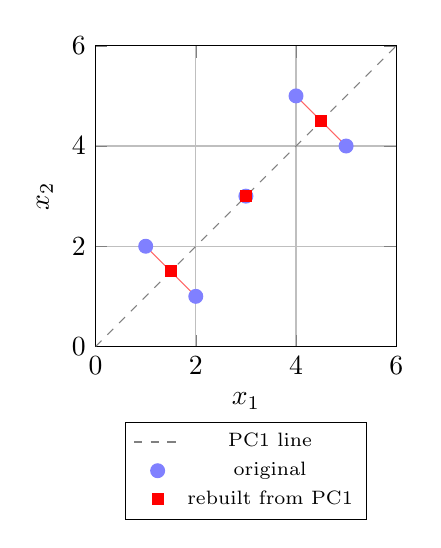
\begin{tikzpicture}
      \begin{axis}[width=5.4cm,height=5.4cm,axis equal,
          xmin=0,xmax=6,ymin=0,ymax=6,grid=major,
          xlabel={$x_1$},ylabel={$x_2$},
          legend style={font=\scriptsize,at={(0.5,-0.25)},anchor=north,legend columns=1}]
        \addplot[gray,dashed,domain=0:6] {x};
        \addlegendentry{PC1 line}
        \addplot[only marks,mark=*,blue!50,mark size=2.5pt]
          coordinates {(1,2)(2,1)(3,3)(4,5)(5,4)};
        \addlegendentry{original}
        \addplot[only marks,mark=square*,red,mark size=2pt]
          coordinates {(1.5,1.5)(3,3)(4.5,4.5)};
        \addlegendentry{rebuilt from PC1}
        \draw[red!60] (axis cs:1,2)--(axis cs:1.5,1.5);
        \draw[red!60] (axis cs:2,1)--(axis cs:1.5,1.5);
        \draw[red!60] (axis cs:4,5)--(axis cs:4.5,4.5);
        \draw[red!60] (axis cs:5,4)--(axis cs:4.5,4.5);
      \end{axis}
    \end{tikzpicture}
  \end{columns}
\end{frame}

% ------------------------------------------------------------
\begin{frame}[fragile]{The same thing in scikit-learn \nb{2}}
\begin{lstlisting}
import numpy as np
from sklearn.decomposition import PCA

X = np.array([[1, 2], [2, 1], [3, 3], [4, 5], [5, 4]])

pca = PCA(n_components=2).fit(X)
pca.mean_                      # [3, 3]
pca.components_                # directions v1, v2 (one per row)
pca.explained_variance_        # [4.5, 0.5]
pca.explained_variance_ratio_  # [0.9, 0.1]

pca1 = PCA(n_components=1).fit(X)
Z = pca1.transform(X)          # the z1 scores, shape (5, 1)
X_hat = pca1.inverse_transform(Z)  # rebuilt readings
\end{lstlisting}
  \vspace{0.3em}
  \small
  \begin{itemize}
    \item \texttt{fit}: learn the directions from the data.
    \item \texttt{transform}: get the scores.
    \item \texttt{inverse\_transform}: go back to the original columns.
  \end{itemize}
\end{frame}

% ------------------------------------------------------------
\begin{frame}{The book example: 200 points \nb{3}}
  \begin{itemize}
    \item 200 random points in 2 columns that move together.
    \item PC1 direction $\approx (0.944,\; 0.329)$
    \item Spread along each direction $\approx (0.763,\; 0.018)$
  \end{itemize}
  \vspace{0.5em}
  Share kept by PC1:
  \[
    \frac{0.763}{0.763 + 0.018} \approx 0.976
  \]
  PC1 alone keeps \textbf{about 98\%} of the information.
  Going from 2 columns to 1 loses very little.

  \vspace{0.8em}
  {\footnotesize The book shows 0.759 instead of 0.763. Older scikit-learn divided by $n$,
  current versions divide by $n-1$ (slide~6). The 98\% is the same either way.}
\end{frame}

% ------------------------------------------------------------
\begin{frame}{Handwritten digits \nb{4}}
  \begin{itemize}
    \item 1,797 images, each $8\times8$ pixels $= $ \textbf{64 numbers} per image.
    \item Each number says how dark one pixel is.
    \item \texttt{PCA(2)} turns the 64 numbers into 2, so each image becomes a dot on a plot.
  \end{itemize}
  \vspace{0.6em}
  \textbf{Why the dots form groups:}
  \begin{itemize}
    \item Two ``0''s darken almost the same pixels, so their 64 numbers are similar.
    \item Similar numbers $\Rightarrow$ similar PC scores $\Rightarrow$ nearby dots.
    \item Digits that share strokes (3, 5, 8) land close and overlap.
  \end{itemize}
  \vspace{0.6em}
  The 2 components keep only about \textbf{28\%} of the information,
  but that is enough to see the groups. PCA never saw the labels.
\end{frame}

% ------------------------------------------------------------
\begin{frame}{How many components to keep? \nb{4}}
  \centering
  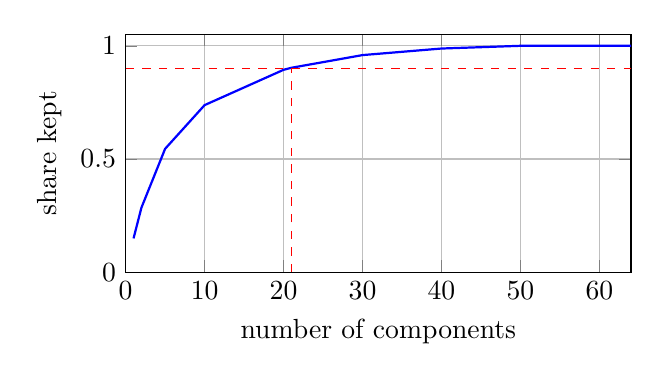
\begin{tikzpicture}
    \begin{axis}[width=8cm,height=4.6cm,
        xlabel={number of components},ylabel={share kept},
        xmin=0,xmax=64,ymin=0,ymax=1.05,grid=major]
      \addplot[blue,thick] coordinates
        {(1,0.149)(2,0.285)(5,0.545)(10,0.738)(20,0.894)(21,0.903)
         (30,0.959)(40,0.988)(50,1.0)(64,1.0)};
      \addplot[red,dashed] coordinates {(0,0.9)(64,0.9)};
      \addplot[red,dashed] coordinates {(21,0)(21,0.903)};
    \end{axis}
  \end{tikzpicture}

  \raggedright
  \begin{tabular}{lcccc}
    \toprule
    Components & 2 & 10 & 21 & 50 \\
    Share kept & 28\% & 74\% & 90\% & $\approx$100\% \\
    \bottomrule
  \end{tabular}
  \vspace{0.5em}

  Pick the number where the curve reaches your target, e.g.\ 90\%.
  \texttt{PCA(0.90)} picks it for you (here: 21).
\end{frame}

% ------------------------------------------------------------
\begin{frame}{PCA as a noise filter \nb{5}}
  \textbf{Idea:} the real pattern sits in the first few components.
  Random noise is spread thinly over all of them.
  \vspace{0.6em}
  \begin{enumerate}
    \item Add random noise to the digit images.
    \item Keep the components that hold 50\% of the information: \texttt{PCA(0.50)} keeps \textbf{12}.
    \item Rebuild the images from those 12 $\Rightarrow$ cleaner digits.
  \end{enumerate}
  \vspace{0.6em}
  Same as the sensors: dropping PC2 removed the disagreement,
  which is where sensor noise shows up.
  \vspace{0.6em}

  A model trained on 12 columns instead of 64 is faster
  and less bothered by noise.
\end{frame}

% ------------------------------------------------------------
\begin{frame}{Eigenfaces \nb{6}}
  \begin{itemize}
    \item Face photos of $62 \times 47$ pixels $= $ about \textbf{2,900 numbers} each.
    \item Keep only the first \textbf{150} components (about 20 times smaller).
    \item They hold just over \textbf{90\%} of the information.
    \item The rebuilt faces are still easy to recognize.
    \item First components capture lighting; later ones capture eyes, nose, mouth.
  \end{itemize}
  \vspace{0.6em}
  Storage per face: $2{,}914 \times 4$ bytes $\approx 11.7$ KB
  vs.\ $150 \times 4 \approx 0.6$ KB.

  \vspace{0.8em}
  {\footnotesize The book uses \texttt{RandomizedPCA}. In current scikit-learn write
  \texttt{PCA(150, svd\_solver="randomized")}.}
\end{frame}

% ------------------------------------------------------------
\begin{frame}{Watch out: units and outliers \nb{7}}
  Same five sensor readings, two common problems.
  \vspace{0.6em}

  \textbf{Units.} Record sensor B in mK instead of K (numbers 1000$\times$ bigger).
  \begin{itemize}
    \item PC1 becomes $\approx (0, 1)$: PCA just follows the bigger numbers.
    \item \textbf{Fix:} standardize each column first (\texttt{StandardScaler}).
          PC1 goes back to $(0.71, 0.71)$ and 90\%.
  \end{itemize}
  \vspace{0.6em}

  \textbf{Outliers.} Add one faulty reading, $(5,\,-10)$.
  \begin{itemize}
    \item PC1 changes from $(0.71,\,0.71)$ to $(-0.10,\; 1.00)$.
    \item One bad point turned ``both sensors'' into ``sensor B only''.
    \item \textbf{Fix:} find and remove or flag bad readings before PCA.
  \end{itemize}
\end{frame}

% ------------------------------------------------------------
\begin{frame}{Other limits}
  \begin{itemize}
    \item \textbf{Straight lines only.} PCA finds straight directions.
          Data that curves needs other methods.
    \item \textbf{New columns are mixes.} PC1 is a blend of the original columns.
          Look at \texttt{components\_} before giving it a name.
    \item \textbf{Large data.} \texttt{PCA(svd\_solver="randomized")}
          finds the first few components quickly.
  \end{itemize}
\end{frame}

% ------------------------------------------------------------
\begin{frame}{Summary \nb{8}}
  \begin{enumerate}
    \item PCA finds the directions where the data spreads the most.
    \item Steps: center, covariance, eigenvectors, project.
    \item Eigenvector = direction; eigenvalue = spread along it.
    \item The share of spread tells you how much you keep.
    \item Uses: shrinking data, plotting, removing noise, preparing model inputs.
  \end{enumerate}
%  \vspace{1em}
%  \textbf{Try it:} make sensor B agree less with sensor A:
%  $x_2 = (4,1,3,2,5)$. Will PC1 keep more or less than 90\%?
%  Work out $\lambda_1$ and $\lambda_2$.
\end{frame}





% ------------------------------------------------------------
\begin{frame}{How many components does PCA produce?}
If you start with \textbf{10 original variables} (10 columns in your table),
PCA will produce \textbf{exactly 10 principal components (PCs)}.

\vspace{0.5em}
There is one component for each original dimension of your data space.

\vspace{0.5em}
\begin{alertblock}{The crucial detail}
What makes PCA useful is that the components are \textbf{not equally important}.
\end{alertblock}
\end{frame}

% ------------------------------------------------------------
\section{Original Variables vs.\ PCs}

\begin{frame}{The difference between original variables and PCs}
The number is the same, but the distribution of the ``information''
(\textbf{variance}) changes completely.

\begin{columns}[T]
\begin{column}{0.48\textwidth}
\begin{block}{Before PCA: original variables}
The information is \textbf{spread across all columns}.
\begin{itemize}
  \item Column 1 holds a little, column 5 holds a little more\ldots
  \item Many columns \textbf{repeat information} from one another
        (they are correlated).
\end{itemize}
\end{block}
\end{column}
\begin{column}{0.48\textwidth}
\begin{exampleblock}{After PCA: principal components}
PCA arranges the new axes in \textbf{order of relevance}.
\begin{itemize}
  \item Each new axis carries as much of the remaining information as possible.
  \item The first PCs hold most of the information.
\end{itemize}
\end{exampleblock}
\end{column}
\end{columns}
\end{frame}

\begin{frame}{How the information is ordered across the PCs}
\begin{itemize}
  \item \textbf{PC1} captures the largest possible share of all the information in the dataset.
  \item \textbf{PC2} takes as much as possible of what is left.
  \item \textbf{PC3} takes a little more\ldots
  \item \ldots and so on, down to the last PCs (such as \textbf{PC9} or \textbf{PC10}),
        which hold almost no relevant information and carry only
        \textbf{mathematical noise}.
\end{itemize}
\end{frame}

% ------------------------------------------------------------
\section{Why does this matter?}

\begin{frame}{Why does this matter? (The key trick)}
Because the last components are almost useless,
\textbf{you can throw them away}.

\vspace{0.5em}
\begin{exampleblock}{Example}
\begin{itemize}
  \item 10 original variables $\rightarrow$ PCA produces 10 PCs.
  \item You may find that \textbf{PC1, PC2, and PC3 together already hold 92\%}
        of all the information in your dataset.
  \item So you \textbf{discard the other 7 axes}.
\end{itemize}
\end{exampleblock}

\vspace{0.5em}
This is how a complex \textbf{10-dimensional} problem becomes a simple
\textbf{3-dimensional} one \textbf{without losing the essence of your data}.
\end{frame}

\end{document}